
% generated by Plantuml 1.2018.00      
\definecolor{plantucolor0000}{RGB}{255,255,255}
\definecolor{plantucolor0001}{RGB}{74,100,132}
\definecolor{plantucolor0002}{RGB}{145,198,255}
\definecolor{plantucolor0003}{RGB}{0,0,0}
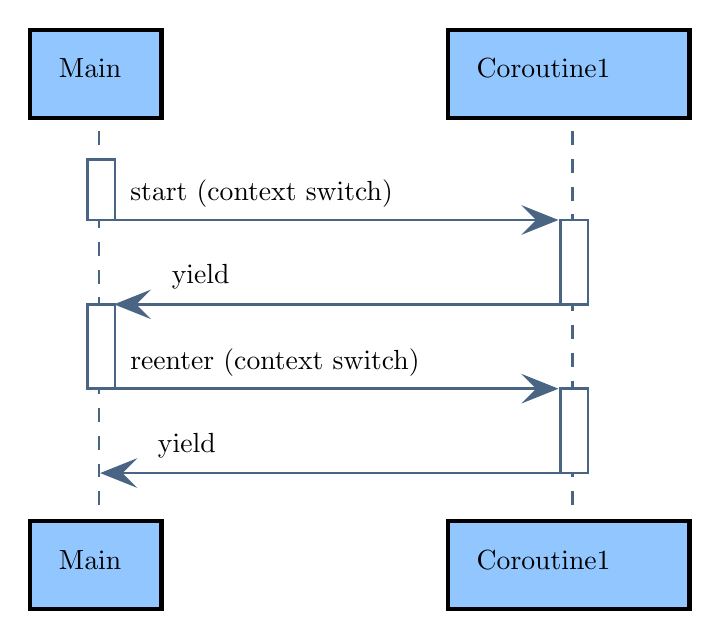
\begin{tikzpicture}[yscale=-1
,pstyle0/.style={color=plantucolor0001,fill=white,line width=1.0pt}
,pstyle1/.style={color=plantucolor0001,line width=1.0pt,dash pattern=on 5.0pt off 5.0pt}
,pstyle2/.style={color=black,fill=plantucolor0002,line width=1.5pt}
,pstyle3/.style={color=plantucolor0001,fill=plantucolor0001,line width=1.0pt}
,pstyle4/.style={color=plantucolor0001,line width=1.0pt}
]
\draw[pstyle0] (28.8pt,49.7461pt) rectangle (38.8pt,71.7461pt);
\draw[pstyle0] (28.8pt,102.2246pt) rectangle (38.8pt,132.7031pt);
\draw[pstyle0] (199.704pt,71.7461pt) rectangle (209.704pt,102.2246pt);
\draw[pstyle0] (199.704pt,132.7031pt) rectangle (209.704pt,163.1816pt);
\draw[pstyle1] (33pt,39.7461pt) -- (33pt,181.6602pt);
\draw[pstyle1] (203.9879pt,39.7461pt) -- (203.9879pt,181.6602pt);
\draw[pstyle2] (8pt,3pt) rectangle (55.6pt,34.7461pt);
\node at (15pt,10pt)[below right,color=black]{Main};
\draw[pstyle2] (8pt,180.6602pt) rectangle (55.6pt,212.4063pt);
\node at (15pt,187.6602pt)[below right,color=black]{Main};
\draw[pstyle2] (158.9879pt,3pt) rectangle (246.4201pt,34.7461pt);
\node at (165.9879pt,10pt)[below right,color=black]{Coroutine1};
\draw[pstyle2] (158.9879pt,180.6602pt) rectangle (246.4201pt,212.4063pt);
\node at (165.9879pt,187.6602pt)[below right,color=black]{Coroutine1};
\draw[pstyle0] (28.8pt,49.7461pt) rectangle (38.8pt,71.7461pt);
\draw[pstyle0] (28.8pt,102.2246pt) rectangle (38.8pt,132.7031pt);
\draw[pstyle0] (199.704pt,71.7461pt) rectangle (209.704pt,102.2246pt);
\draw[pstyle0] (199.704pt,132.7031pt) rectangle (209.704pt,163.1816pt);
\draw[pstyle3] (187.704pt,67.7461pt) -- (197.704pt,71.7461pt) -- (187.704pt,75.7461pt) -- (191.704pt,71.7461pt) -- cycle;
\draw[pstyle4] (33.8pt,71.7461pt) -- (193.704pt,71.7461pt);
\node at (40.8pt,53.7461pt)[below right,color=black]{start (context switch)};
\draw[pstyle3] (49.8pt,98.2246pt) -- (39.8pt,102.2246pt) -- (49.8pt,106.2246pt) -- (45.8pt,102.2246pt) -- cycle;
\draw[pstyle4] (43.8pt,102.2246pt) -- (203.704pt,102.2246pt);
\node at (55.8pt,84.2246pt)[below right,color=black]{yield};
\draw[pstyle3] (187.704pt,128.7031pt) -- (197.704pt,132.7031pt) -- (187.704pt,136.7031pt) -- (191.704pt,132.7031pt) -- cycle;
\draw[pstyle4] (33.8pt,132.7031pt) -- (193.704pt,132.7031pt);
\node at (40.8pt,114.7031pt)[below right,color=black]{reenter (context switch)};
\draw[pstyle3] (44.8pt,159.1816pt) -- (34.8pt,163.1816pt) -- (44.8pt,167.1816pt) -- (40.8pt,163.1816pt) -- cycle;
\draw[pstyle4] (38.8pt,163.1816pt) -- (203.704pt,163.1816pt);
\node at (50.8pt,145.1816pt)[below right,color=black]{yield};
\end{tikzpicture}